\section{Bash à sable}

Le but de ce TP d'introduction est de sa familiariser avec l'environnement Unix Ubuntu et de voir quelques outils, notamment \bashcmd, que vous utiliserez par la suite dans les TPs. Nous allons voir comment~:
\begin{itemize}
\item créer/supprimer des fichiers/répertoires (récursivement éventuellement)
\item écrire un script bash pour manipuler des fichiers, changer ses droits
\item rechercher/installer des packages
\item ...
\end{itemize}

\subsection{Prise en main}

Pendant tout les TPs, nous allons utiliser deux outils: la console (ou terminal) et l'éditeur \emacs; c'est depuis un terminal que les scripts seront exécutes et ceux-ci seront écrits avec l'éditeur de texte \emacs. \\

Sous l'environnement Gnome 3, pour afficher la liste des applications disponibles, vous pouvez déplacer le curseur de souris dans le coin en haut à gauche de votre écran ou bien appuyer sur la touche du windows du clavier si elle existe. Vous pouvez alors directement saisir ``Terminal'' et cliquer sur l'application qui s'affiche dans la liste.\\

Le terminal qui s'affiche alors devrait ressembler à la fenêtre ci-dessous.

\begin{figure}[htbp]
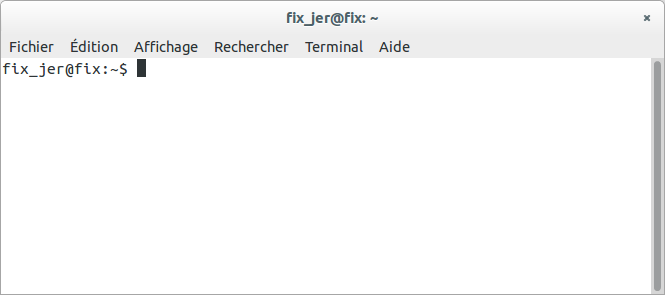
\includegraphics[width=0.5\columnwidth]{Figs/terminal.png}
\caption{Terminal (ou console)}
\end{figure}

C'est depuis ce type de fenêtre (vous pouvez lancer plusieurs instances de terminal, ou même plusieurs onglets) que nous allons exécuter nos scripts, créer des répertoires, etc...

\subsection{Navigation dans le système de fichier}

Il y a un certain de commandes à connaître pour pouvoir naviguer dans le système de fichier, testez les commandes suivantes depuis un terminal~:
\begin{itemize}
\item \ls : pour lister le contenu du répertoire courant
\item \ls /chemin/vers/un/repertoire : pour lister le contenu du répertoire passé en argument
\item \pwd : pour connaître le chemin du répertoire courant
\item \cd : pour changer de répertoire (``\cd ..'' permet de remonter d'un répertoire, ``\cd \textasciitilde'' permet de se rendre à son \emph{home})
\item \mkdir : pour créer un répertoire (ou une hiérarchie de répertoire avec l'option ``-p'')
\item \myrm : pour supprimer un fichier (ajoutez l'option ``-r'' pour supprimer un répertoire)
\end{itemize}

\textbf{Créez} vous un répertoire sur votre home (accessible par ``\cd \textasciitilde'') dans lequel vous stockerez les scripts que vous allez développer pendant cet électif.

\subsection{Rechercher/Installer des packages}

L'une des forces de Linux est de pouvoir facilement\footnote{en général} installer des logiciels. Il y a principalement deux façons de le faire: 1) à partir du code source, 2) à partir de paquets binaires pré-compilés pour votre distribution. La deuxième façon de faire est la plus facile et c'est celle à laquelle on va s'intéresser. Quelle que soit la distribution, il existe un système de gestion des paquets binaires: apt pour Ubuntu, yum pour fedora, ...; Nous n'allons pas le voir pendant ces TP, mais sachez qu'il est extrêmement facile d'installer de nouveaux logiciels (de nouveaux paquets) avec ces gestionnaires de paquet. Par exemple, sous Fedora, vous pourriez regarder les commandes suivantes~:
\begin{itemize}
\item yum search : pour chercher un paquet
\item yum install : pour l'installer
\item yum remove : pour le supprimer
\end{itemize}
L'installation de nouveaux paquets se faisant en général dans les chemins /usr/lib, /usr/bin, /usr/include, il faut être superutilisateur pour pouvoir procéder à ces installations.


\subsection{Éditer du code, un document, etc.. avec \emacs}

Pour éditer du code vous avez plusieurs possibilités. Une est d'utiliser des IDE dédiés. Une autre est de faire cela avec un éditeur de texte comme \emacs. \emacs est un peu plus qu'un éditeur de texte, il apporte les fonctionnalités les plus utiles à un développeur dont la coloration syntaxique et l'indentation. Il est également \emph{customizable} et il existe des modes qui sont chargés automatiquement en fonction de l'extension du fichier que vous éditez, par exemple~:
\begin{itemize}
\item python-mode si l'extension du fichier est .py
\item c++-mode si l'extension est .cpp ou .cc
\item sh-mode si l'extension est .sh (pour un script bash)
\item tex-mode si l'extension est .tex (pour des fichiers \LaTeX)
\item ...
\end{itemize}
Ces modes consistent notamment en une coloration syntaxique particulière et des menus particuliers. Pour vous en rendre compte, lancez depuis un terminal les commandes suivantes~:
\begin{itemize}
\item emacs titi.py \&
\item emacs titi.cpp \&
\item emacs titi.sh \&
\item emacs titi.tex \&
\end{itemize}
Vous trouverez plus d'informations sur emacs p.\pageref{sec:emacs}.\\

Le symbole \& permet de lancer une commande en tâche de fond. Vous récupérez alors la main dans votre terminal. Essayez de lancer une des commandes sans la faire suivre de \& et essayez de lister le répertoire courant avec \ls. Si vous avez lancé une application sans la mettre en tâche de fond, vous pouvez la mettre en tâche de fond en utilisant, \textbf{depuis le terminal ou la commande est lancée}, la combinaison de touches Ctrl+Z puis taper bg [Entrée].

\subsection{Bashons un peu}

Au travers des différents TP qui suivent, l'idée est de construire des programmes en mettant bout à bout des petits programmes qui réalisent des fonctions élémentaires. On va voir un peu plus loin ce qu'on entends par là. Le langage de programmation bash va nous servir de glu pour assembler ces petits programmes. Je vous propose donc dans un premier temps de voir quelques notions de base en Bash et d'aller petit à petit vers la programmation par flux. A la fin de ce TP, vous devriez~:
\begin{itemize}
\item connaître quelques programmes de base et accéder à leur documentation
\item être capable d'écrire de petits scripts Bash et de les assembler
\end{itemize}


\paragraph{Mon premier script bash:}

A l'aide de \emacs, éditez un fichier \bash{hello.sh}. Ajoutez le code ci-dessous dans ce fichier.

\cprotect\encadreUtilisation{
\begin{verbatim}
#!/bin/bash

echo "hello world!"
\end{verbatim}
}
Vous pouvez maintenant exécuter ce script, en lançant depuis un terminal \bash{sh hello.sh}. Il devrait s'afficher ``hello world!''.\\

Il est possible de rendre ce script exécutable. Les droits d'écriture, lecture, exécution d'un fichier sont détaillés dans la section~\ref{sec:permissions}. Par défaut le script bash n'a pas les droits d'exécution. Vérifiez les permissions sur le script en appelant \bash{ls -l hello.sh}. On peut alors ajouter des droits d'exécution à l'aide de la commande \bash{chmod u+x hello.sh}. On ajoute ici les droits d'exécution (+x) pour l'utilisateur courant (u), c'est à dire vous. On le verra pas pendant cet électif, mais les droits permettent de garantir qu'on ne fait pas n'importe quoi sous linux; il faut par exemple passer explicitement administrateur (qui s'appelle super-utilisateur dans le monde unix) pour pouvoir modifier du système dans /usr; Vous devriez maintenant pouvoir exécuter votre script \bash{./hello.sh}. La première ligne du script "\#!/bin/bash" indique quel interpréteur utiliser pour évaluer le script\footnote{On verra plus tard d'autres interpréteurs; par exemple, lorsqu'on écrira des scripts Python, on mentionnera "\#!/usr/bin/python"}. C'est grâce à cette ligne que Linux sait qu'il faut exécuter le script avec sh, sachant que ``/bin/bash'' est le chemin vers le programme à utiliser pour interpréter le script.


\paragraph{Passer des arguments à un script bash et structures de contrôle:}

Lorsqu'un script \bashcmd est appelé avec des arguments, ces arguments sont accessibles par les variables \$i. La variable \$0 contient, par convention, le nom du script exécuté. La variable \$\# contient le nombre d'arguments passés au script. Testez le script ci-dessous qui permet d'afficher les arguments passés à un script.

 \cprotect\encadreUtilisation{
\begin{verbatim}
#!/bin/bash

echo "J'ai reçu $# arguments"

if [ $# != 0 ]
then
    echo "Liste des arguments : "
    for i in $@; do
	echo "$i"
    done
else
    echo "donc rien à lister"
fi

echo "J'ai reçu $# arguments"
\end{verbatim}
}

Vous pouvez tester le script en lui passant ou non des arguments.


\paragraph{Appeler des fonctions depuis un script bash:}

On peut appeler des fonctions, lancer des scripts, etc.. finalement exécuter n'importe quelle commande Unix depuis un script bash. Dans le script ci-dessous, on utilise les fonctions basename et dirname qui retournent respectivement le nom d'un fichier passé en argument et le répertoire ou ce fichier se trouve.

\cprotect\encadreUtilisation{
\begin{verbatim}
#!/bin/bash

echo "Je m'exécute depuis le répertoire `pwd`"
echo "Le script $0 s'appelle `basename $0` et se trouve dans le répertoire `dirname $0`"

\end{verbatim}
}

%% \paragraph{Ecrire des fonctions dans un script bash:}
%% On peut aussi définir ses propres fonctions dans un script bash. Supposons qu'on souhaite disposer d'une fonction qui compte le nombre de caractères d'une chaîne de caractères, on peut alors définir le script suivant~:
%% \cprotect\encadreUtilisation{
%% \begin{verbatim}
%% #!/bin/bash

%% function compte {
%%     if [ $# != 1 ]
%%     then
%% 	echo "Oups: nombre invalide d'arguments" 1>&2
%%     else
%% 	echo -n $1 | wc -c 
%%     fi;
%% }

%% # Un appel sans arguments
%% compte
%% # Un appel avec des arguments 
%% compte "ma chaine de caractères"
%% \end{verbatim}
%% }
%% On a déjà vu que la variable "\$0" contient le nombre d'arguments passés à un script, mais il contient également, dans le contexte d'une fonction, le nombre d'arguments passés à la fonction. On s'assure donc que la fonction reçoit bien un argument. On verra un peu plus tard ce que signifie "1>\&2". \\

%% La commande qui calcule le nombre de caractères d'une chaîne est "wc -m" (vérifiez le en regardant "man wc"). On lui passe une chaîne de caractère dans l'entrée standard (on en parle juste après) grâce à la commande \echo. Le résultat est renvoyé sur la sortie standard.


\paragraph{Entrée et sorties standards}
\label{p:entrees_sorties_standards}

Quand l'exécution d'une commande affiche du texte dans la console, c'est que la commande a écrit dans au moins l'un des deux canaux qu'on appelle ``sortie standard''(\emph{stdout}) et ``erreur standard''(\emph{stderr}). Ces deux canaux sont des canaux de sortie. Un programme dispose également d'un canal d'entrée, "l'entrée standard" (\emph{stdin}). On représente sur la figure \ref{fig:Stdstreams} un exemple de programme pour lequel le clavier est envoyé sur l'entrée standard et les sortie standard 

\begin{figure}[htbp]
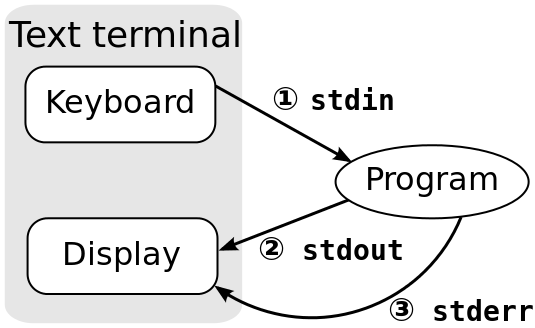
\includegraphics[width=0.5\columnwidth]{Figs/Stdstreams.png}
\caption{\label{fig:Stdstreams}Entrée standard, sortie standard et sortie d'erreur}
\end{figure}

Le terminal dans lequel vous saisissez du texte est un programme qui lit les informations saisies au clavier et les affiche. On va voir juste après qu'il est possible de chaîner des programmes de telle sorte que la sortie standard d'un programme serve d'entrée standard à un autre et ainsi construire un ``pipeline'' de traitement. 

\paragraph{Enchaîner des scripts bash: filtres et ``pipe''}

La philosophie des outils GNU consiste à écrire des outils très spécifiques et à les combiner. La combinaison de ces outils se fait par le caractère ``|'' (le pipe). La structure générale d'un pipeline est de connecter une source à un puits en appliquant successivement plusieurs filtres. Comme on va le voir, ces filtres peuvent être des commandes Bash mais rien ne vous empêche d'en écrire dans d'autres langages (comme Python). On a dit précédemment qu'une commande pouvait écrire dans sa sortie standard. En connectant deux commandes par le pipe, par exemple commande1 | commande2, la sortie standard de commande1 est connectée sur l'entrée standard de commande2. commande2 peut alors travailler sur les informations envoyées par commande1. On peut donc combiner plusieurs commandes très spécifiques pour construire un programme plus intéressant que les commandes individuelles. Par exemple, la commande \du permet de calculer l'espace occupé par des fichiers, la commande \sort permet de trier les lignes d'un fichier, on peut alors facilement lister les fichiers/répertoires du répertoire courant par ordre croissant de taille~:
\begin{center}
du * | sort -n
\end{center}
Si on ne veut afficher que les 10 plus gros fichiers/répertoires, il suffit d'afficher les 10 dernières éléments~:
\begin{center}
du * | sort -n | tail -10 
\end{center}


\subsection{Ecrire un script lisant l'entrée standard}

Pour lire depuis l'entrée standard (et on le fera souvent par la suite durant le TP), on utilisera la commande \readcmd. 

\cprotect\encadreUtilisation{
\begin{verbatim}
#!/bin/bash
while read -r ligne
do
    echo "Ligne lue : $ligne"
done
\end{verbatim}
}

Sauvegardez le script ci-dessous dans un fichier \bash{read\_input.sh} et testez le ~:
\begin{exempleResultat}
bash:\$ cat read_input.sh | ./read\_input.sh
\end{exempleResultat}

\begin{center}

\end{center}

\subsection{Avoir des informations sur l'utilisation d'une commande}

Sous linux, on peut facilement accéder à une page de manuel d'une commande à l'aide de la commande \man exécutée depuis un terminal. Par exemple, pour avoir plus d'informations sur l'utilisation de la commande \mkdir permettant de créer des répertoires, on utilisera~:

\begin{exempleResultat}
bash:\$ man mkdir
\end{exempleResultat}
On navigue alors dans le texte qui s'affiche à l'aide des flêches directionnelles. Pour quitter la page de manuelle, il suffit de presser la touche q. 

%Voir les commandes : tee et 

\vfill 
\newpage
